\documentclass{article}
\usepackage[utf8]{inputenc}
\usepackage{tikz}


\title{Mondrian}
\author{francesconowell }
\date{September 2020}

\begin{document}

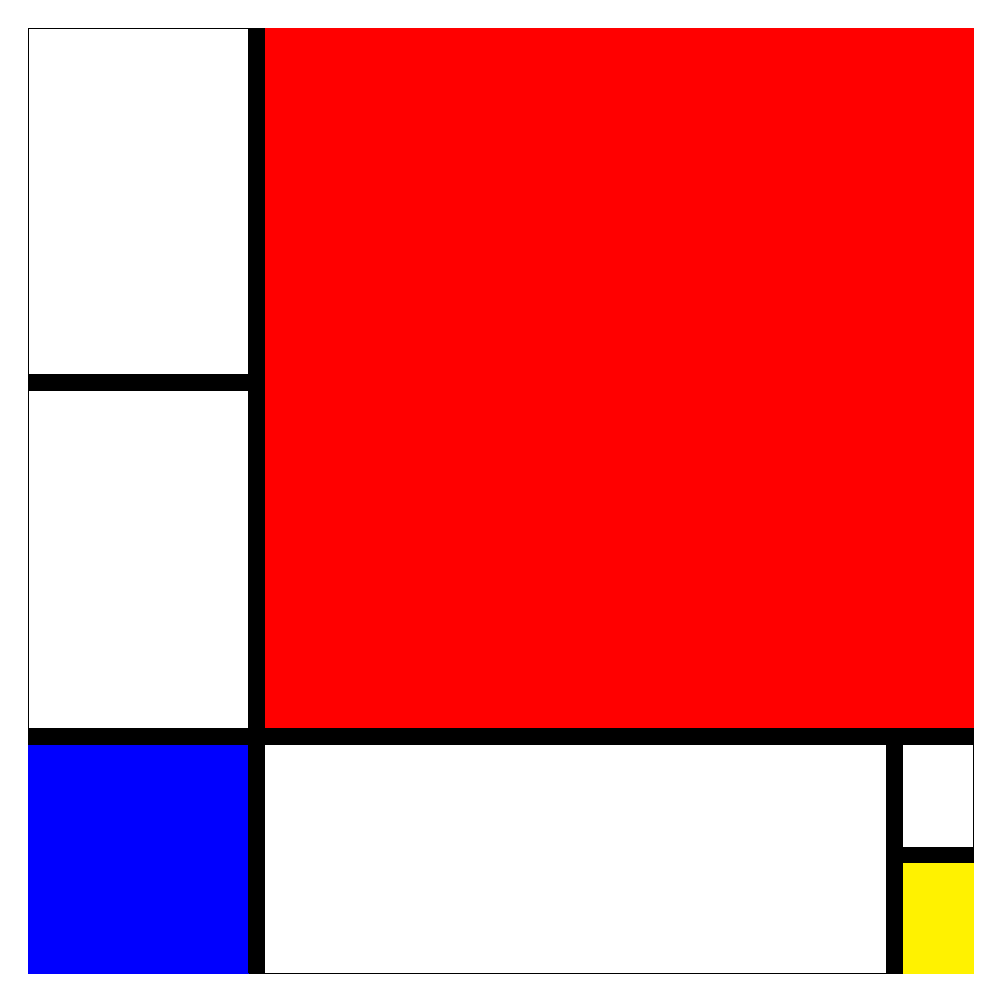
\begin{tikzpicture}
\draw (0,0) -- (12,0) -- (12,12) -- (0,12) -- (0,0);
\filldraw [red] (3,3) -- (12,3) -- (12,12) -- (3,12) -- (3,3);
\filldraw [blue] (0,0) -- (3,0) -- (3,3) -- (0,3) -- (0,0);
\filldraw [yellow] (11,0) -- (12,0) -- (12,1.5) -- (11,1.5) -- (11,0);
\filldraw [black] (2.8,0) -- (3,0) -- (3,12)--(2.8,12) -- (2.8,0);
\filldraw [black] (0,2.9) -- (12,2.9)--(12,3.1)--(0,3.1) --(0,2.9);
\filldraw [black] (0,7.4) --(3,7.4)--(3,7.6)--(0,7.6)--(0,7.4);
\filldraw [black]  (10.9,0) --(11.1,0) -- (11.1,2.9)-- (10.9,2.9)--(10.9,0);
\filldraw [black] (11,1.4)--(12,1.4)--(12,1.6)--(11,1.6)--(11,1.4);
 
\end{tikzpicture}
\\ 

Piet Mondrian, "Composition in Red, Blue and Yellow", 1929 
\end{document}
